% latex table generated in R 3.2.2 by xtable 1.8-0 package
% Wed Jan 27 11:17:04 2016
% \vspace{-1.5cm}
{\setlength{\tabcolsep}{0.3em}}
{\renewcommand{\arraystretch}{1}}% for the vertical padding
% \footnotesize
\begin{tabular}{
  l>{\centering\arraybackslash}%
  m{1.5cm}>{\centering\arraybackslash}%
  m{3.0cm}>{\centering\arraybackslash}%
  m{1.7cm}cccc>{\centering\arraybackslash}%
  m{2.7cm}>{\centering\arraybackslash}%
  m{2.7cm}>{\centering\arraybackslash}%
  m{1.1cm}cc%
}%
\toprule
  & 
  & \multicolumn{6}{c}{\textbf{Network Properties}}
  & \multicolumn{2}{c}{\textbf{Complexity} }
  & \multicolumn{3}{c}{\textbf{Algorithms}}
  \\
%-------------------------------------------------------------------------------
%-------------------------------------------------------------------------------
 \cmidrule(lr){3-8}\cmidrule(lr){9-10}\cmidrule(lr){11-13}
  & \multirow[c]{-2}*{\textbf{Problem}}
  & \multicolumn{1}{c}{Graph Structure}
  & \multicolumn{1}{c}{Example}
  & \screentextcolor{GENERATOR}{$\fmagnitude{\glssymbol{generators}}$} 
  & \screentextcolor{CONSUMER}{$\fmagnitude{\glssymbol{consumers}}$}
  & \screentextcolor{SUSCEPTANCE}{$\glssymbol{susceptance}$}
  & \screentextcolor{CAPACITY}{$\glssymbol{capacity}$}
  & \multicolumn{1}{c}{Hardness}
  & \multicolumn{1}{c}{Reference}
  & \multicolumn{1}{c}{Name} 
  & \multicolumn{1}{c}{\screentextcolor{SUSCEPTANCE}{$\glssymbol{susceptance}$}}
  & \multicolumn{1}{c}{\screentextcolor{CAPACITY}{$\glssymbol{capacity}$}}
  \\
%-------------------------------------------------------------------------------
%-------------------------------------------------------------------------------
 \midrule\addlinespace
%-------------------------------------------------------------------------------
%-------------------------------------------------------------------------------
\rowcolor{Table-Line-Marker}
%-------------------------------------------------------------------------------
1\label{ch:switching:sec:exploit_structural_characteristics:tbl:tree}
& \gls{mtsfp} and~\gls{otsp}
& tree graphs
& \raisebox{-0.5cm}[0pt][0pt]{
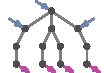
\includegraphics{switchplacement/figures/graph_structure-tree.pdf}%
}
& \screentextcolor{GENERATOR}{$\infty$}
& \screentextcolor{CONSUMER}{$\infty$}
& \screentextcolor{SUSCEPTANCE}{--}
& \screentextcolor{CAPACITY}{--}
& polynomial-time solvable
& 
\cref{ch:network-analyzes:sec:mathematical-model:lem:pf-matrix-is-tum}, 
\cref{ch:facts:thm:fvs},
\cref{ch:foundations:sec:graph-theoretical-flows} p.\ 
\pageref{ch:foundations:sec:graph-theoretical-flows:para:maximum-flow-problem}
& \gls{mf} & \screentextcolor{SUSCEPTANCE}{$\infty$} &
\screentextcolor{CAPACITY}{$\infty$}
\\\addlinespace\addlinespace
% 
2\label{ch:switching:sec:exploit_structural_characteristics:tbl:penrose_minor}
& \gls{mtsfp} and~\gls{otsp}
& penrose-minor-free graphs
& \raisebox{-0.5cm}[0pt][0pt]{
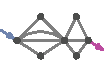
\includegraphics{switchplacement/figures/graph_structure-penrose_minor_free_graph.pdf}}
& \screentextcolor{GENERATOR}{1}
& \screentextcolor{CONSUMER}{1}
& \screentextcolor{SUSCEPTANCE}{--}
& \screentextcolor{CAPACITY}{--}
& polynomial-time solvable
& \cref{ch:switching:sec:exploit_structural_characteristics,ch:switching:sec:computing_one_dtp}
& \gls{dtp}
& \screentextcolor{SUSCEPTANCE}{$\infty$}
& \screentextcolor{CAPACITY}{$\infty$}
\\\addlinespace\addlinespace
% 
\rowcolor{Table-Line-Marker}
%-------------------------------------------------------------------------------
& \gls{mtsfp}
& series-parallel
& % --
& % --
& % --
& \screentextcolor{SUSCEPTANCE}{$\infty$}
& \screentextcolor{CAPACITY}{$\infty$}
& % --
& \parencite{Koc16}
& % --
& % --
& % --
\\
% 
\rowcolor{Table-Line-Marker}
%-------------------------------------------------------------------------------
\multirow{-2}*{3}
\label{ch:switching:sec:exploit_structural_characteristics:tbl:series_parallel}
& and~\gls{otsp}% \acrshort{mtsf} and~\acrshort{ots}
& graphs % series-parallel graphs
& \multirow{-2}*{\raisebox{-0.5cm}[0pt][0pt]{%{-\totalheight}
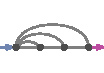
\includegraphics{switchplacement/figures/graph_structure-series_parallel_graph.pdf}}}
& \multirow{-2}*{\screentextcolor{GENERATOR}{1}}
& \multirow{-2}*{\screentextcolor{CONSUMER}{1}}
& \cellcolor{KITpalegreen15}\screentextcolor{SUSCEPTANCE}{$\infty$}
& \cellcolor{KITpalegreen15}\screentextcolor{CAPACITY}{$1$}
& \multirow{-2}*{\NP-hard}
& \cellcolor{KITpalegreen15}\cref{ch:switching:sec:complexity}
& \multirow{-2}*{--}
& \multirow{-2}*{\screentextcolor{SUSCEPTANCE}{--}} 
& \multirow{-2}*{\screentextcolor{CAPACITY}{--}}
\\\addlinespace\addlinespace
% 
4\label{ch:switching:sec:exploit_structural_characteristics:tbl:cactus}
& \gls{mtsfp} and~\gls{otsp}
& cacti with maximum degree of~$3$
& \raisebox{-0.5cm}[0pt][0pt]{%{-\totalheight}
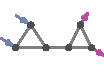
\includegraphics{switchplacement/figures/graph_structure-cacti_graph.pdf}}
& \screentextcolor{GENERATOR}{$\infty$}
& \screentextcolor{CONSUMER}{$\infty$}
& \screentextcolor{SUSCEPTANCE}{1}
& \screentextcolor{CAPACITY}{$\infty$}
& \NP-hard
& \parencite{Leh14}
& \gls{maxst} (see~\cref{ch:switching:sec:approximation_algorithm_on_cacti})
& \screentextcolor{SUSCEPTANCE}{--}
& \screentextcolor{CAPACITY}{--}
\\\addlinespace\addlinespace
% 
\rowcolor{Table-Line-Marker}
%-------------------------------------------------------------------------------
5\label{ch:switching:sec:exploit_structural_characteristics:tbl:2_level_tree}
& \gls{mtsfp} and~\gls{otsp}
& 2-level trees
& \raisebox{-0.5cm}[0pt][0pt]{%{-\totalheight}
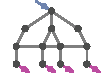
\includegraphics{switchplacement/figures/graph_structure-two_level_tree.pdf}}
& \screentextcolor{GENERATOR}{1}
& \screentextcolor{CONSUMER}{$\infty$}
& \screentextcolor{SUSCEPTANCE}{$\infty$}
& \screentextcolor{CAPACITY}{$\infty$}
& \NP-hard
& \parencite{Leh14}
& --
& \screentextcolor{SUSCEPTANCE}{--}
& \screentextcolor{CAPACITY}{--}
\\\addlinespace\addlinespace
% 
6\label{ch:switching:sec:exploit_structural_characteristics:tbl:plane_graph}
& \gls{mtsfp} and~\gls{otsp}
& planar graph with~$\max$ degree of~$3$
& \raisebox{-0.5cm}[0pt][0pt]{%{-\totalheight}
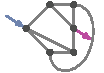
\includegraphics{switchplacement/figures/graph_structure-plane_graph.pdf}}
& \screentextcolor{GENERATOR}{1}
& \screentextcolor{CONSUMER}{1}
& \screentextcolor{SUSCEPTANCE}{$\infty$}
& \screentextcolor{CAPACITY}{1}
& strongly~\NP-hard
& \parencite{Leh14}
& --
& \screentextcolor{SUSCEPTANCE}{--}
& \screentextcolor{CAPACITY}{--}
\\\addlinespace\addlinespace
% 
\rowcolor{Table-Line-Marker}
%-------------------------------------------------------------------------------
& \gls{mtsfp}
& % --
& % --
& \screentextcolor{GENERATOR}{2}
& \screentextcolor{CONSUMER}{2}
& % --
& % --
& % --
& \parencite{Leh14}
& % --
& % --
& % --
\\
% 
\rowcolor{Table-Line-Marker}
%-------------------------------------------------------------------------------
\multirow{-2}*{7}
\label{ch:switching:sec:exploit_structural_characteristics:tbl:arbitrary_graph}
& \cellcolor{KITpalegreen15}\gls{otsp} 
& \multirow{-2}*{arbitrary graphs}
& \multirow{-2}*{\raisebox{-0.5cm}[0pt][0pt]{%{-\totalheight}

\includegraphics{switchplacement/figures/graph_structure-arbitrary_graph.pdf}}}
& \cellcolor{KITpalegreen15}\screentextcolor{GENERATOR}{1}
& \cellcolor{KITpalegreen15}\screentextcolor{CONSUMER}{$\infty$}
& \multirow{-2}*{\screentextcolor{SUSCEPTANCE}{$\infty$}}
& \multirow{-2}*{\screentextcolor{CAPACITY}{$\infty$}}
& \multirow{-2}*{non-\APX}
& \cellcolor{KITpalegreen15}\parencite{Leh14}
& \multirow{-2}*{--}
& \multirow{-2}*{\screentextcolor{SUSCEPTANCE}{--}} 
& \multirow{-2}*{\screentextcolor{CAPACITY}{--}}
\\\addlinespace\addlinespace
% 
%-------------------------------------------------------------------------------
%-------------------------------------------------------------------------------
   \bottomrule
\end{tabular}
